\section{Functional Connectivity Analysis with fMRI Data}\label{sec:realdata}


We demonstrate the advantage of thresholding based spectral density estimators for visualization and interpretation in functional connectivity analysis among different brain regions of a human subject using resting state fMRI data. This data is part of a study involving 51 subjects (29.6 $\pm$ 8.6 years of age, 35 males) that suffered from mild traumatic brain injury (TBI). Magnetic resonance imaging (MRI) data and neuropsychological data were collected at 1 week, 1 month, 6 months and 12 months post-injury. TBI is defined as Glasgow Coma Scale of 13-15 at injury, loss of consciousness less than 30 minutes and post-traumatic amnesia less than 24 hours. More  details are available in  \cite{Kuceyeski2018functional}. 
%We focus on the MRI collected at 1 month and 6 month because most recovery in this cohort occurred between these two time points \citep{Kuceyeski2018functional}. 
% {\color{red} Here you can reference my bioRxiv paper from this year that shows most cognitive recovery occurred between 1 and 6 months in this dataset.}

%After removal of observations collected at 1 week and 12 months, the dataset is balanced but not complete. There were a total of 27 subjects (29.1 $\pm$ 8.1 years of age, 21 males) with both imaging and  neuro-psychological measurements at 1 and 6 months. The same MRI sequences for demographic matched controls (28.6 $\pm$ 8.8 years of age, 25 males) were also collected for comparison.

\begin{figure}
    \centering
    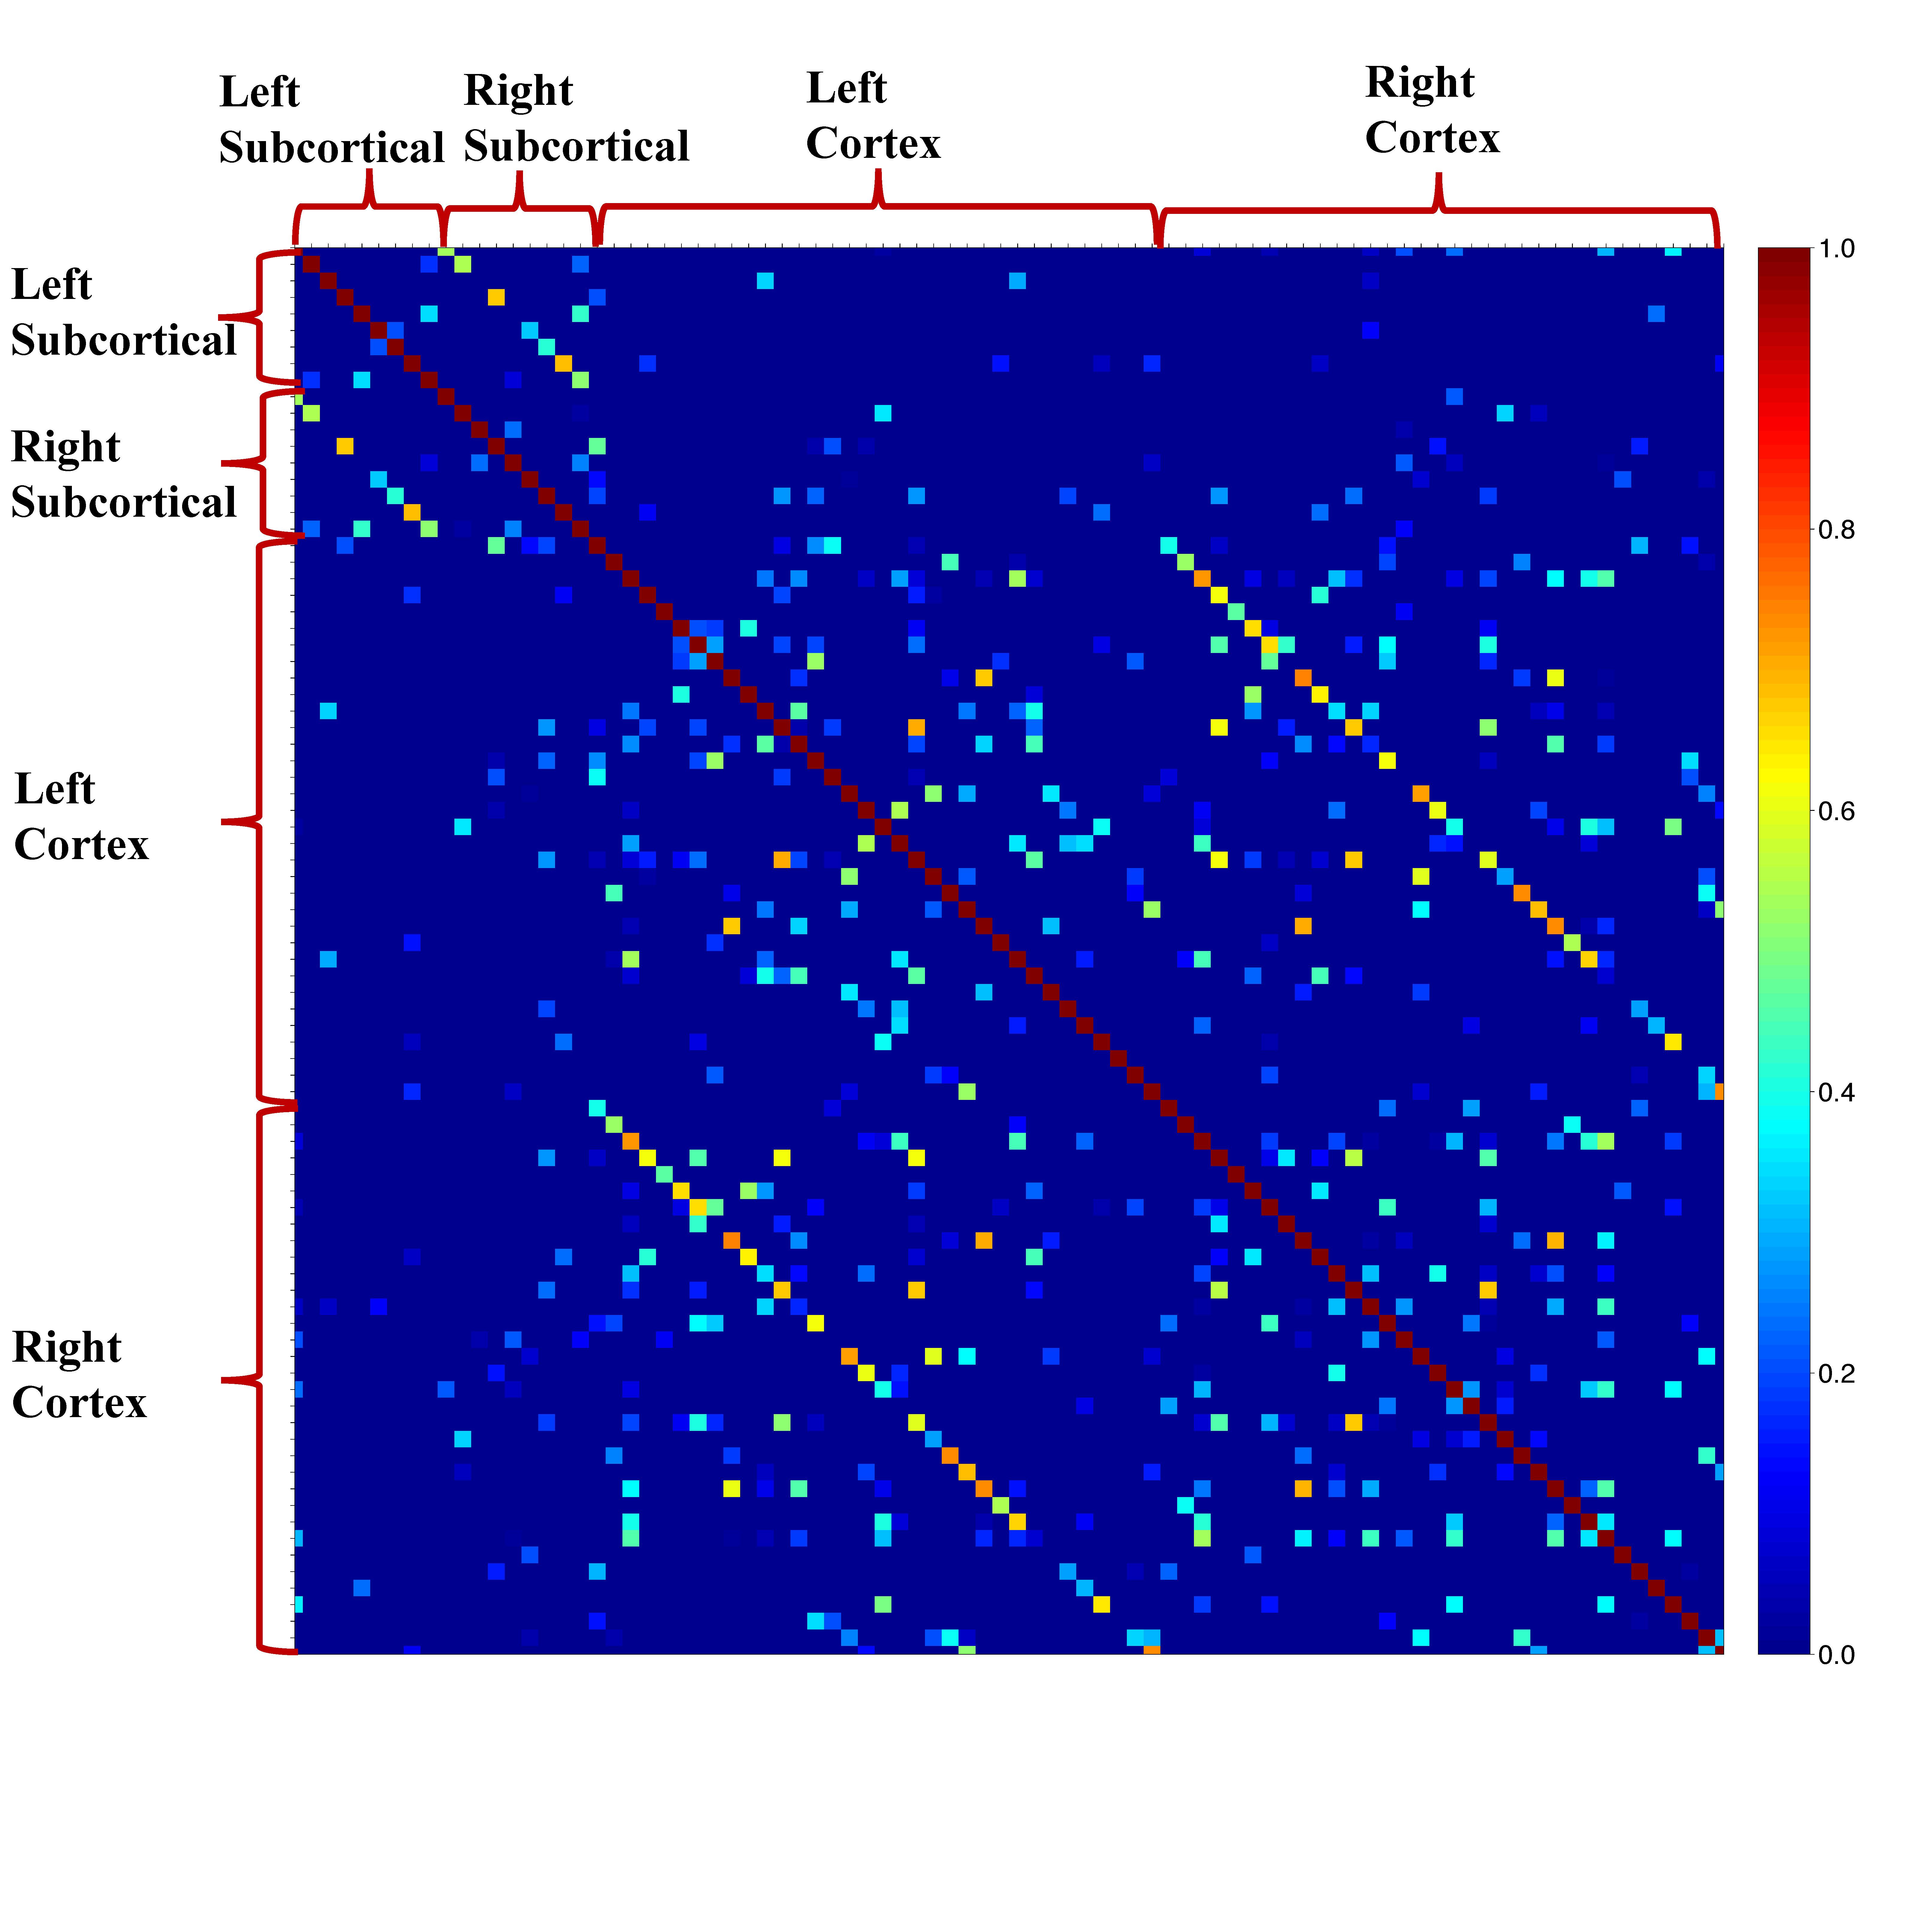
\includegraphics[width=0.48\textwidth]{img/al_hm_nl.pdf}
    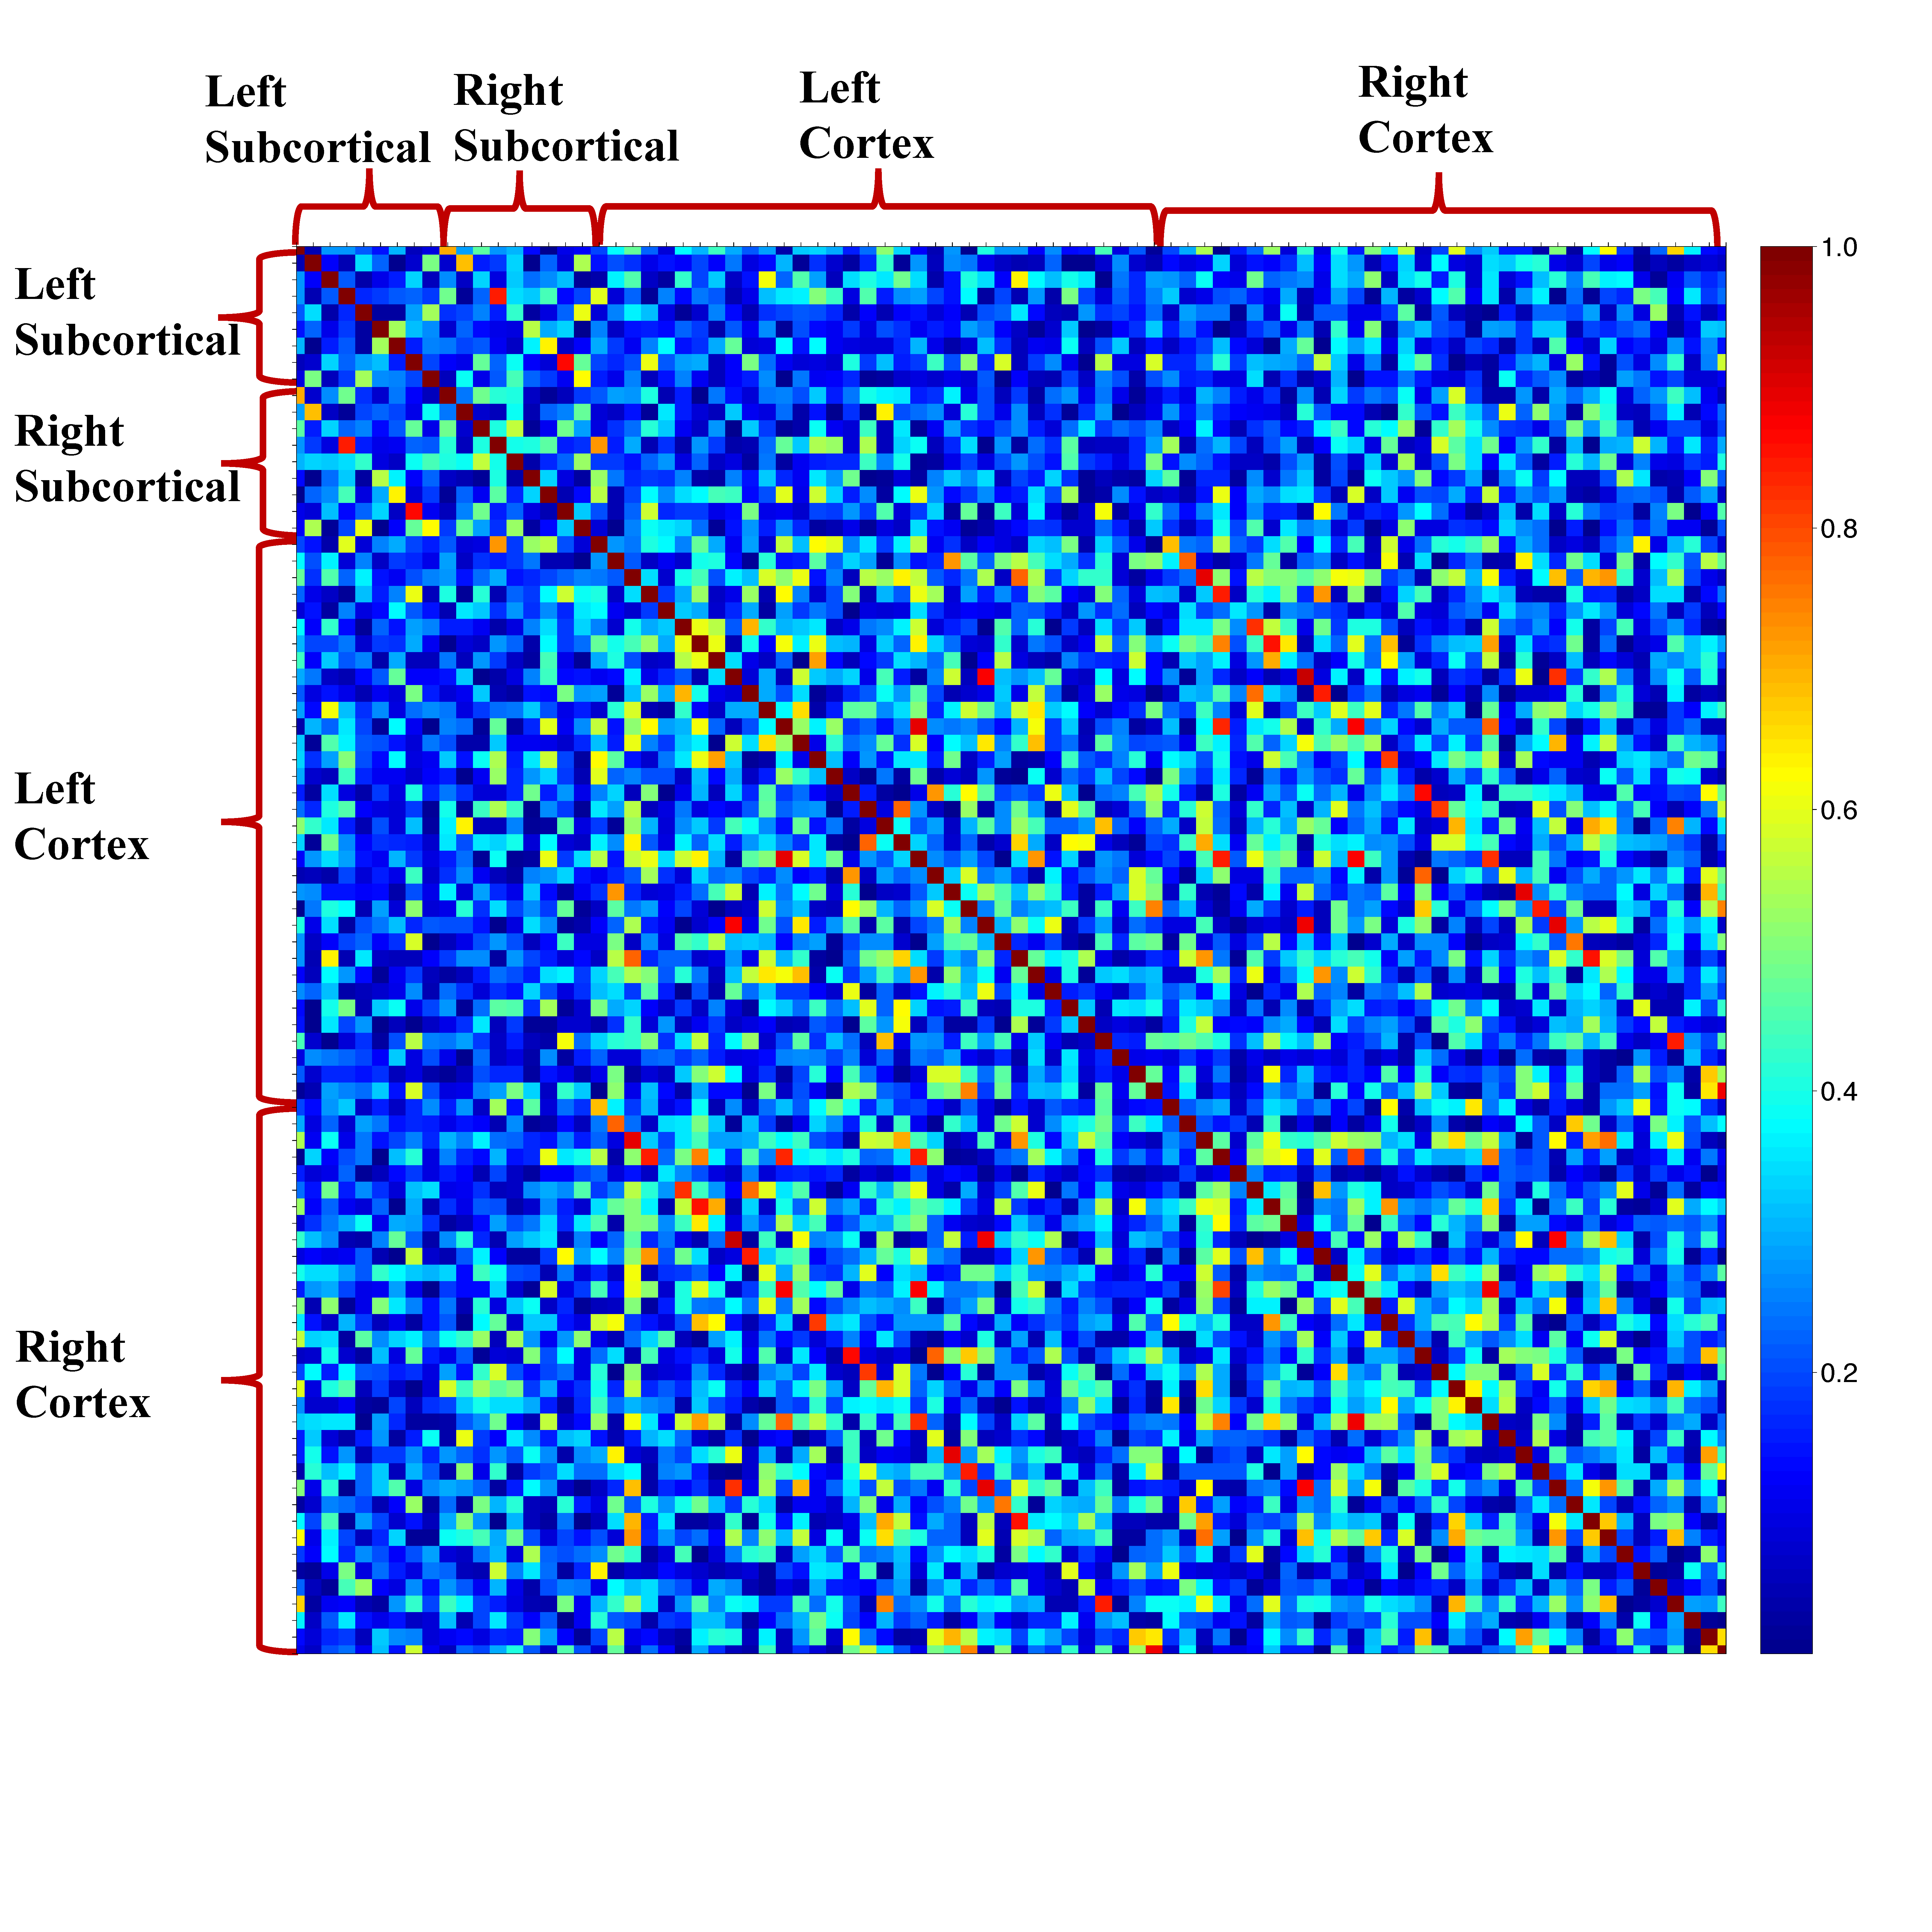
\includegraphics[width=0.48\textwidth]{img/sh_hm_nl.pdf}
    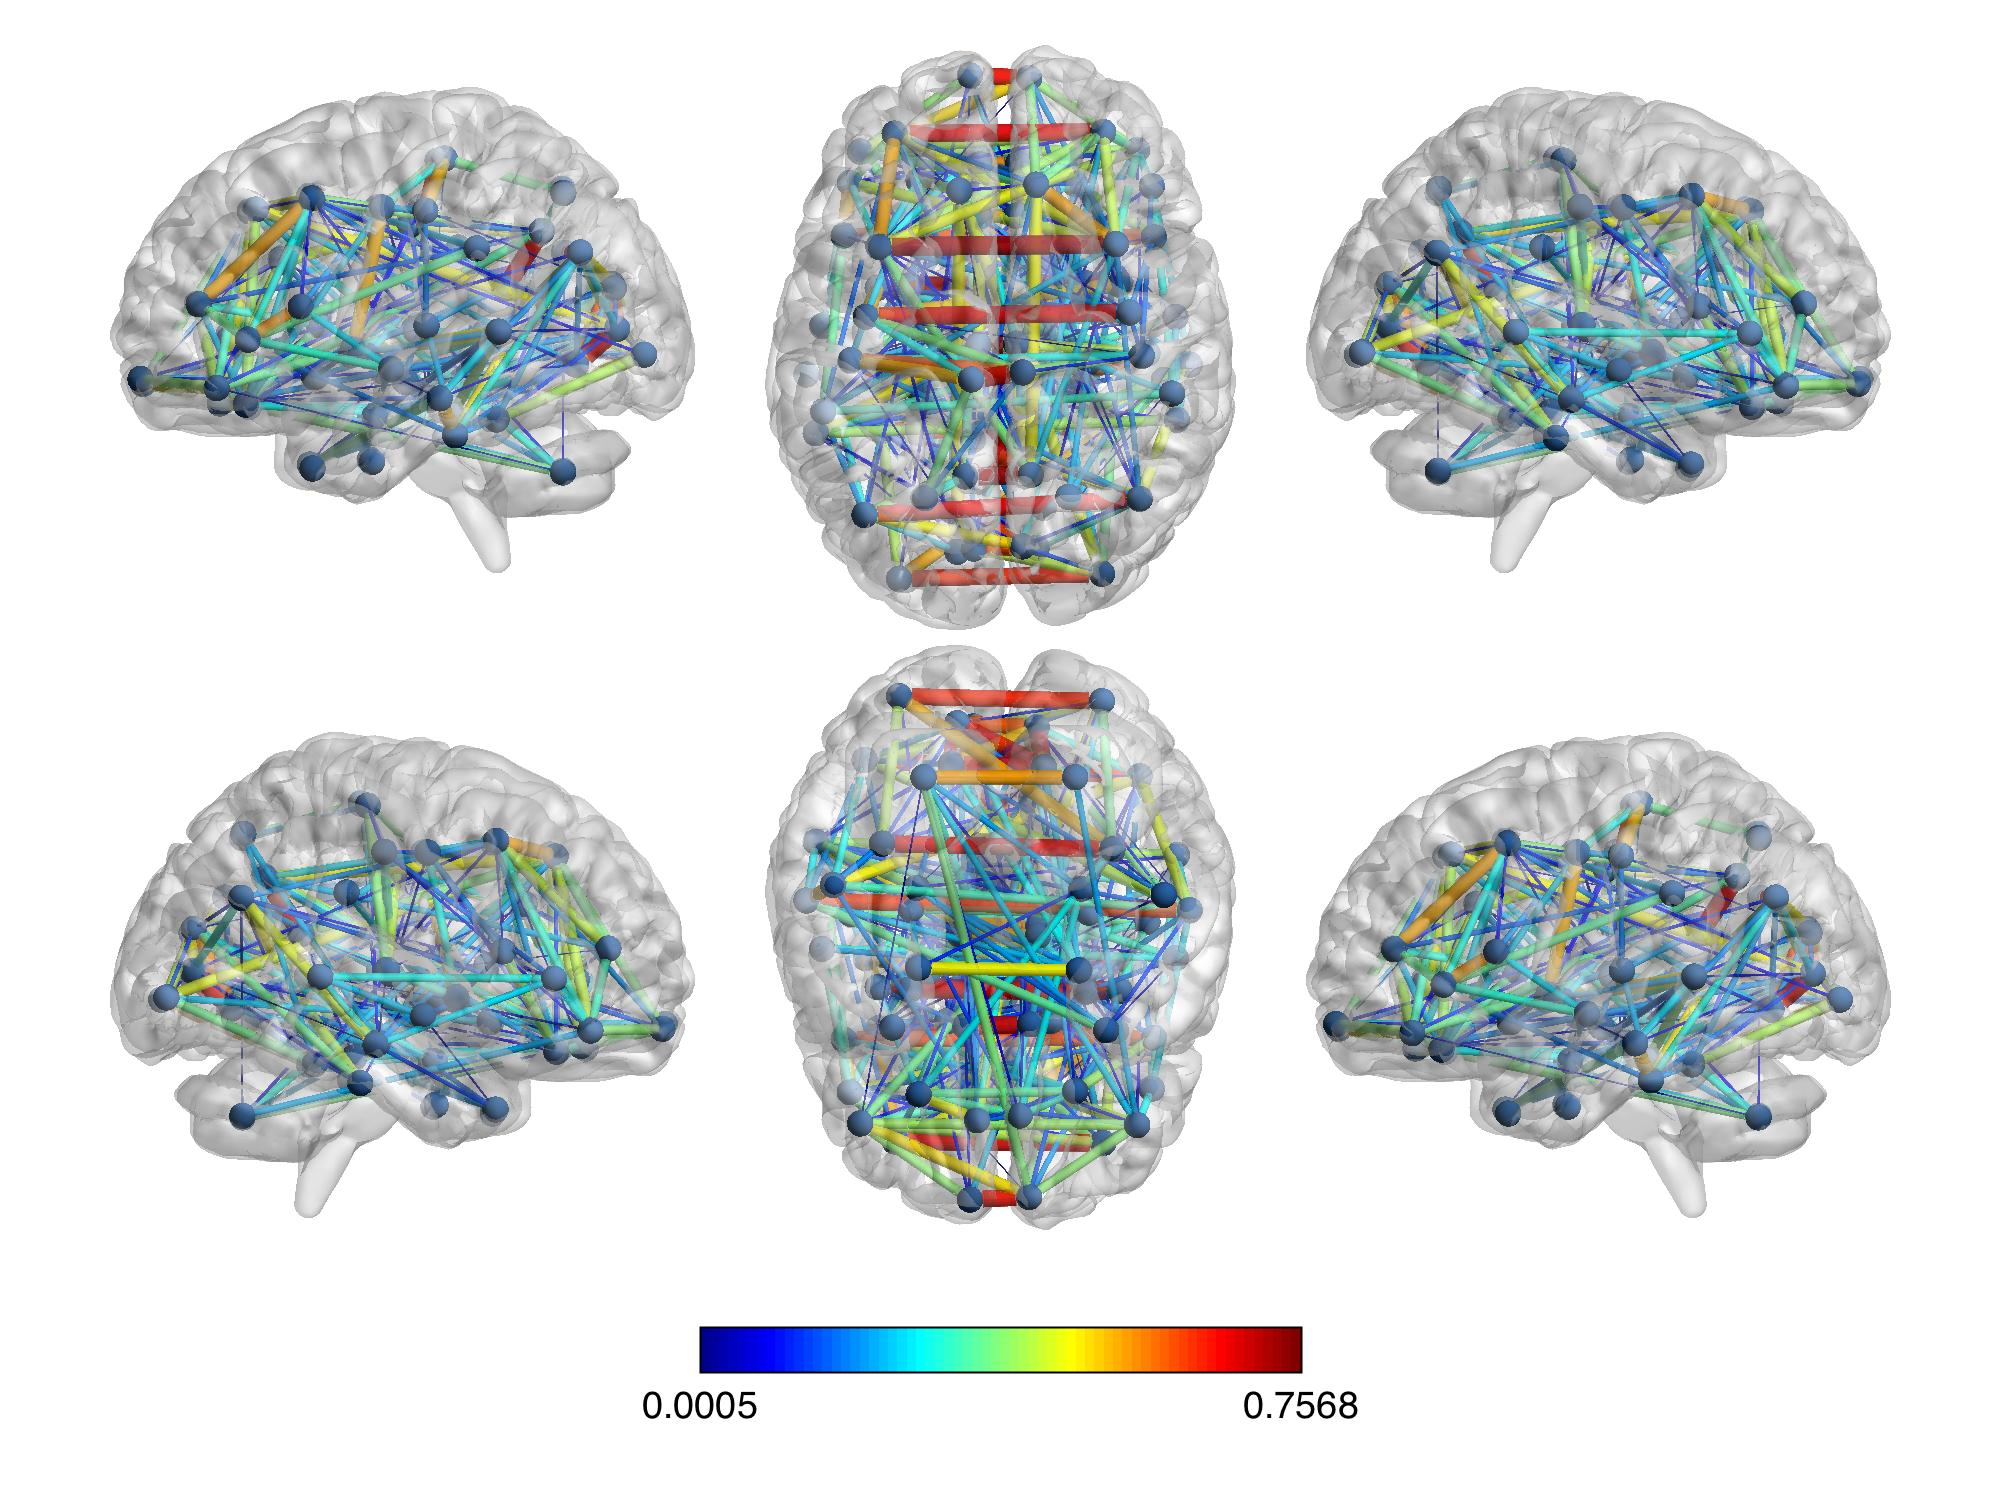
\includegraphics[width=0.95\textwidth]{img/al_c.jpg}
    \caption{[top]: Heat maps of absolute coherence matrices (at frequency $0$) obtained from  spectral density estimated using [top left] adaptive lasso thresholding  and [top right] a shrinkage method. [bottom]: Absolute coherence network among brain regions obtained using adaptive lasso and visualized using BrainNet Viewer. The coherence network estimated by adaptive lasso retains known biological patterns, including presence of bilateral homologues, i.e. strong connectivity between same ROIs in the left and right parts of brain.}
    \label{fig:realdata}
\end{figure}


A 3T GE Signa EXCITE scanner was used to  acquire the MRIs, which included structural scans (FSPGR T1, $1\times 1 \times 1$ mm$^3$ voxels) and resting-state functional magnetic resonance imaging (fMRI) (7 min, $3.4 \times 3.4 \times 4.0$ mm$^3$ voxels, 2 sec sampling rate). The MRIs were processed by parcellating the gray matter into $p=86$ anatomical regions of interest (ROIs) using the semi-automated FreeSurfer software \citep{fischl2000measuring}. Cortical and subcortical parcellations and the fMRI time series data were then used in the construction of coherence based functional connectivity (FC) networks. The adjacency matrix of FC network captures the similarity of the neuronal activation over time between pairs of ROIs. 

We calculated coherence matrices at frequency $0$ using adaptive lasso thresholding (with $\eta = 2$) and shrinkage of averaged periodograms. The smoothing span was chosen by setting $m=\sqrt{n}$, and the tuning parameters in our sample-splitting algorithm were selected as in our simulation studies. 

\textit{Results}: In Figure \ref{fig:realdata}, we show an example of the FC coherence network for a particular TBI patient using our proposed adaptive lasso thresholding (top left) and the same patient's FC network estimated using the shrinkage method (top right) of \citep{bohm2009shrinkage} that does not perform automatic coherence selection. One of the many issues with using fMRI data is the spurious functional connections that arise from the method's abundant noise (due to instrumentation and physiology). It is often preferable in a clinical context to filter out this noise, but it is not currently done in a universally accepted and statistically principled way. As shown in the top panel of Figure \ref{fig:realdata}, the coherence matrix estimated by adaptive lasso thresholding obviously is more sparse in nature compared to the one from shrinkage method, while maintaining known physiological connections. For example, we see strong FC in the bilateral homologues (the same ROI in the left versus right hemisphere), which are known to have strong functional connections \citep{zuo2010growing}. This is even more readily apparent in the bottom panel of Figure \ref{fig:realdata} where we see strong connections between the same ROI in the left and right sides of the brain. Other than the bilateral homologues, the left and right precuneus, isthmus cingulate, lingual gyrus and pericalcarine have prominent connections to many regions (see Figures \ref{fig:realdatafullalasso} and \ref{fig:realdatafullshrinkage} in Appendix \ref{appendix:more_tables}). The precuneus, which plays a role in visual, sensorimotor, and attentional information processing, is central to resting-state (task negative) fMRI networks detected using correlation analysis \citep{Utevsky14}. Additionally, the isthmus cingulate, part of the posterior cingulate cortex, is known to be highly functionally connected to many regions across the brain at rest \citep{FRANSSON20081178}. In addition, we see a stronger FC between the left and right homologues in the subcortical ROIs (upper left corner) than between subcortical and cortical ROIs. It is interesting to note that while some of these connections are also strong in the shrinkage based coherence matrix estimate, it is not easy to separate them from other moderately strong coherences between brain regions.



